\chapter{Resultater}
Der er i dette projekt udarbejdet en prototype, som kan være med til at undersøge muligheden for en automatiseret metode at isolerer langerhanske øer. Der er udviklet et færdig system som har potentiale til at isolere langerhanske øer, det vil sige at produktet kan isolere plantefrø som er brugt i en simuleringsvæske. Derfor er de mekaniske og elektriske dele på plads, til videre undersøgelser af konceptet. I projektet er der også opnået en billedebehandling der understøtter konceptet, i kraft af hurtigheden af processeringen af de simuleret billeder. Der er brugt simuleret billeder, da det indkøbte kamera ikke har været af tilstrækkelig kvalitet.
\section{Det færdige system}

\subsection{brugergrænseflade}
\fxnote{vil du skrive dette Esager?}

\subsection{Tidsinterval mellem kamera og ventil}
Tidsintervallet mellem kameraet og ventilen er en vigtig faktor i systemet. Det er   intervallet fordi det beskriver tiden fra, at kameraet har detekteret en ø til den er ved ventilen, hvor den skal isoleres. En estimatsion er beregnet igennem nedenstående formler. Kravet fra kunden hedder 30 øer i minuttet, derfor skal systemet som minimum have en flow hastighed på 11,25 ml/min. Se formel \ref{eg:ohastighed} for udregningen.

\begin{align}
\frac{\text{Opløsningsstørelse}}{\text{Antal øer i opløsning}} = \frac{150}{400}*30 = 11,25ml/min
\label{eg:ohastighed}
\end{align}(\textit{jf. Søren Gregersen})

For at sorteringen af langerhanske øer sker, kræver det en beregning af hastigheden det tager for en langerhansk ø, at komme fra kameraet til ventilen. Det kan estimeres ud fra det beregnede volumen af slangen, i mellem kameraet og ventil \ref{eg:slangevolume}.

\begin{align}
V=\pi*r^2*h=\pi*\frac{\SI{51}{\micro\metre}}{2}*5cm=0,04ml
\label{eg:slangevolume}
\end{align}

 Det vil sige at med et flow på 11,25ml/min, som er beregnet ud fra formlen \ref{eg:ohastighed}. Der ud fra kan det tiden fra kamera til ventil beregnes ved formelen \ref{eq:tidsintervallet}. 
 
\begin{align}
\frac{11,25}{60}=0,1875\text{ ml pr sek}\to\frac{0,04}{0,1875}=0.213\text{ sekunder}=213ms
\label{eq:tidsintervallet}
\end{align} 

i følge bilaget til ventilen har den et volume 27 ul

\begin{align}
\text{Tid for udtømning af ventilen} = \frac{ventil volume}{ml pr. sekund}=\frac{27ul}{0,1875}=144ms
\label{eq:ventilvolume}
\end{align}

Fra de overstående beregninger kan det observeres, at tidsintervallet mellem kamera og ventilen er 213 millisekunder. Ud fra dette tidsinterval skal systemets tid fra, at kameraet har detekteret en ø til at ventilen kan åbne trækkea fra. Ligeledes skal den omvendte tid med ventilens tid til at lukke også trækkes fra. Ifølge databladet har ventilen en åbningstid op til 20ms og en lukketid på op til 30ms.
\begin{align}
Timerdelay=213ms-70ms-40ms=103ms
\label{eq:timerdelay}
\end{align} 

\fxnote{tiderne skal testes i en integrationstest}
Dette er tiden der skal gå fra kameraet har detekteret en ø til, den samme ø er ved ventilen. Der er implementeret et timer delay til dette i softwaren. For at være sikker på at øen bliver isoleret, er der implementeret endnu et timer delay der beskriver åbningstiden for ventilen. Til dette skal ventilen åbne lidt før og lukke lidt efter. Derfor bør tidsintervallet mellem kamera og ventil differentieres med 20ms og 20ms efter. i formel \ref{eq:ventilvolume} skal der bruge 144ms for at tømme ventilens volume, der er timer delayet til åbningstiden for ventilen på 184ms. 
Åbningstiden er et kompromis, fordi det ikke er favorable at det eksokrine væv kommer over i den isoleret beholder, men samtidigt skal sandsynligheden for at ventilen er åben når øen kommer være så høj som mulig.
\fxnote{meget af det bør flyttes ned i dokumentationen}

\subsection{Hardwaren}
Den overordnet funktion af hardwaren er, at pumpe opløsningsvæsken forbi kameraet hen til ventilen i \textit{wastebeholderen} eller beholderen til de isoleret langerhanske øer. For at fremvise projektets færdige resultater, er der skrevet en kort beskrivelse af komponenterne og deres funktioner nedenfor.

\subsubsection{Styreenheden} 
Til at kontroller hardware komponenterne i systemet er der brugt en styreenhed i form af et arduino udviklingsboard, som er velegnet til producering af prototyper som i dette projekt. Udover at styre komponenterne sikre arduinoen også integrationen, mellem computeren og hardwaren. Derfor er det styreenheden der kontroller flow hastigheden, styrken af kameralyset samt åbning og lukning af ventilen. Se afsnit XX i projektdokumentationen for uddybende dokumentation for design og implementering af styreenheden.

\subsubsection{Motordriveren}
Motordriveren bruges i systemet til at forsyne pumpen, ventil og kameralyset. Motordriveren er nødvendig da Arduinoen ikke kan trække strøm nok til, at trække de nævnte komponenter. Motordriveren består af en L293D\fxnote{er det for specifikt?}, som efterligner signalerne modtaget af arduinoen og videre giver dem til komponenterne, men med forsyning igennem en strømforsyning der i modsætning til arduinoen kan levere den nødvendige strøm. Ved PWM signalet hæver motordriveren amplituden, med strømforsyningensspænding i stedet for arduinoensspænding. Se afsnit XX i projektdokumentationen for uddybende dokumentation for design og implementering af motordriveren.

\subsubsection{Ventil}
Ventilen skal kort sagt isolere de langerhanske øer, når kameraet har detekteret en ø. For at være sikker på at isoleringen er succesfuld er der implementeret en tidsforsinkelse på ventil når den er åben. Denne tid er en prioritering for det er uønsket, at få rest vævet med i den isoleret ø beholder. Tiden er i projektet beregnet og senere estimeret ud fra forsøg med simuleringsvæsken. Se afsnit XX i projektdokumentationen for uddybende dokumentation for design og implementering af ventilen.

\subsubsection{Pumpe}
Pumpens opgave er at skabe et flow i slanger og der ved drive opløsningsvæsken forbi kameraet og hen til ventilen. I projektet er der brugt en peristaltisk pumpe, der skaber et flow ved at sammenpresse slangen ved rotation. Denne pumpe type skaber et stabilt flow med mulighed for variable hastighed, ved hjælp af PWM forsyning fra arduinoen igennem motordriveren. Se afsnit XX i projektdokumentationen for uddybende dokumentation for design og implementering af pumpen.

\subsubsection{Vægtcellen}
Vægtcellen vejer opløsningsbeholderen og stopper systemet når der ikke er mere væske i beholderen. Vægtcellens output er i millivolt hvilket har medført at det skulle forstærkes, for at ADCens opløsning på arduionen kunne udnyttes fuldt ud. Derfor er der brugt en operationsforstærker til dette formål. Yderligere er vægtcellen kalibreret i softwaren ved hjælp af lineær regression. Der kan læses mere omkring implementeringen af vægtcellen i afsnit XX for design og implementering af komponenten, både for software og hardware.

\subsubsection{Kameralyset}
I prototypen er der brugt fire lysdioder til, at have fuldstændig kontrol over lyset til kameraet. Det er erfaret igennem enhedstest af kameraet, at lyset som påvirker kameraet er meget vigtig for detektionen af øerne. Se afsnit XX i projektdokumentationen for yderligere dokumentation af kameralyset.

\subsection{Kameraet}
Det indkøbte kamera har vist sig ikke at være af tilstrækkelig kvalitet igennem en enhedstest. Der kunne ikke skelnes mellem det eksokrine væv og de langerhanske øer. Der kan læses mere om enhedstesten af kameraet i afsnit XX i projektdokumentationen. For at komme videre i projektet er billederne brugt til at simulere opløsningsvæsken med langerhanske øer i gennem en slanger, er billederne af isoleret øer brugt, hvor billederne er taget med kameraet. \fxnote{skriv noget mere!} 

\subsection{Simulering af kamera}
Til at generere et billedsæt, der simulerer langerhanske øer, er der udviklet et Matlab script. Scriptet består overordnet af 3 faser. Den første fase består i at segmentere langerhanske øer udfra et billede og oprette dem som en maske. I anden fase laves en maske bestående af ekstra væv, mens der i tredje fase simuleres flow. I den sidste fase gemmes også de enkelte billeder i formatet .png. De enkelte faser er nærmere beskrevet under deres afsnit. Der anvendes 3 billeder til grundlag for genereringen. Det ene billede viser isolerede øer. Det andet billede viser opløsningen indeholdende øer og ekstra væv. Det sidste billede er et baggrundsbillede uden øer eller ekstra væv. Dette billede anvendes som baggrund for de genererede billeder. Billederne der er valgt stammer fra det indkøbte kamera. Grunden til de kan anvendes som grundlag for genereringen af billeder, på trods af kameraets utilstrækkelige kvalitet, er at øerne og det ekstra væv er adskilt i de enkelte billeder. Dette muliggør en seperat segmentering af øer og væv, som  herefter kan sammensættes til billeder der ligger tæt op af det man observerer gennem et almindeligt mikroskop. De 3 billeder er vist herunder.

\begin{figure}[htbp] \centering
\begin{minipage}[b]{0.3\textwidth} \centering
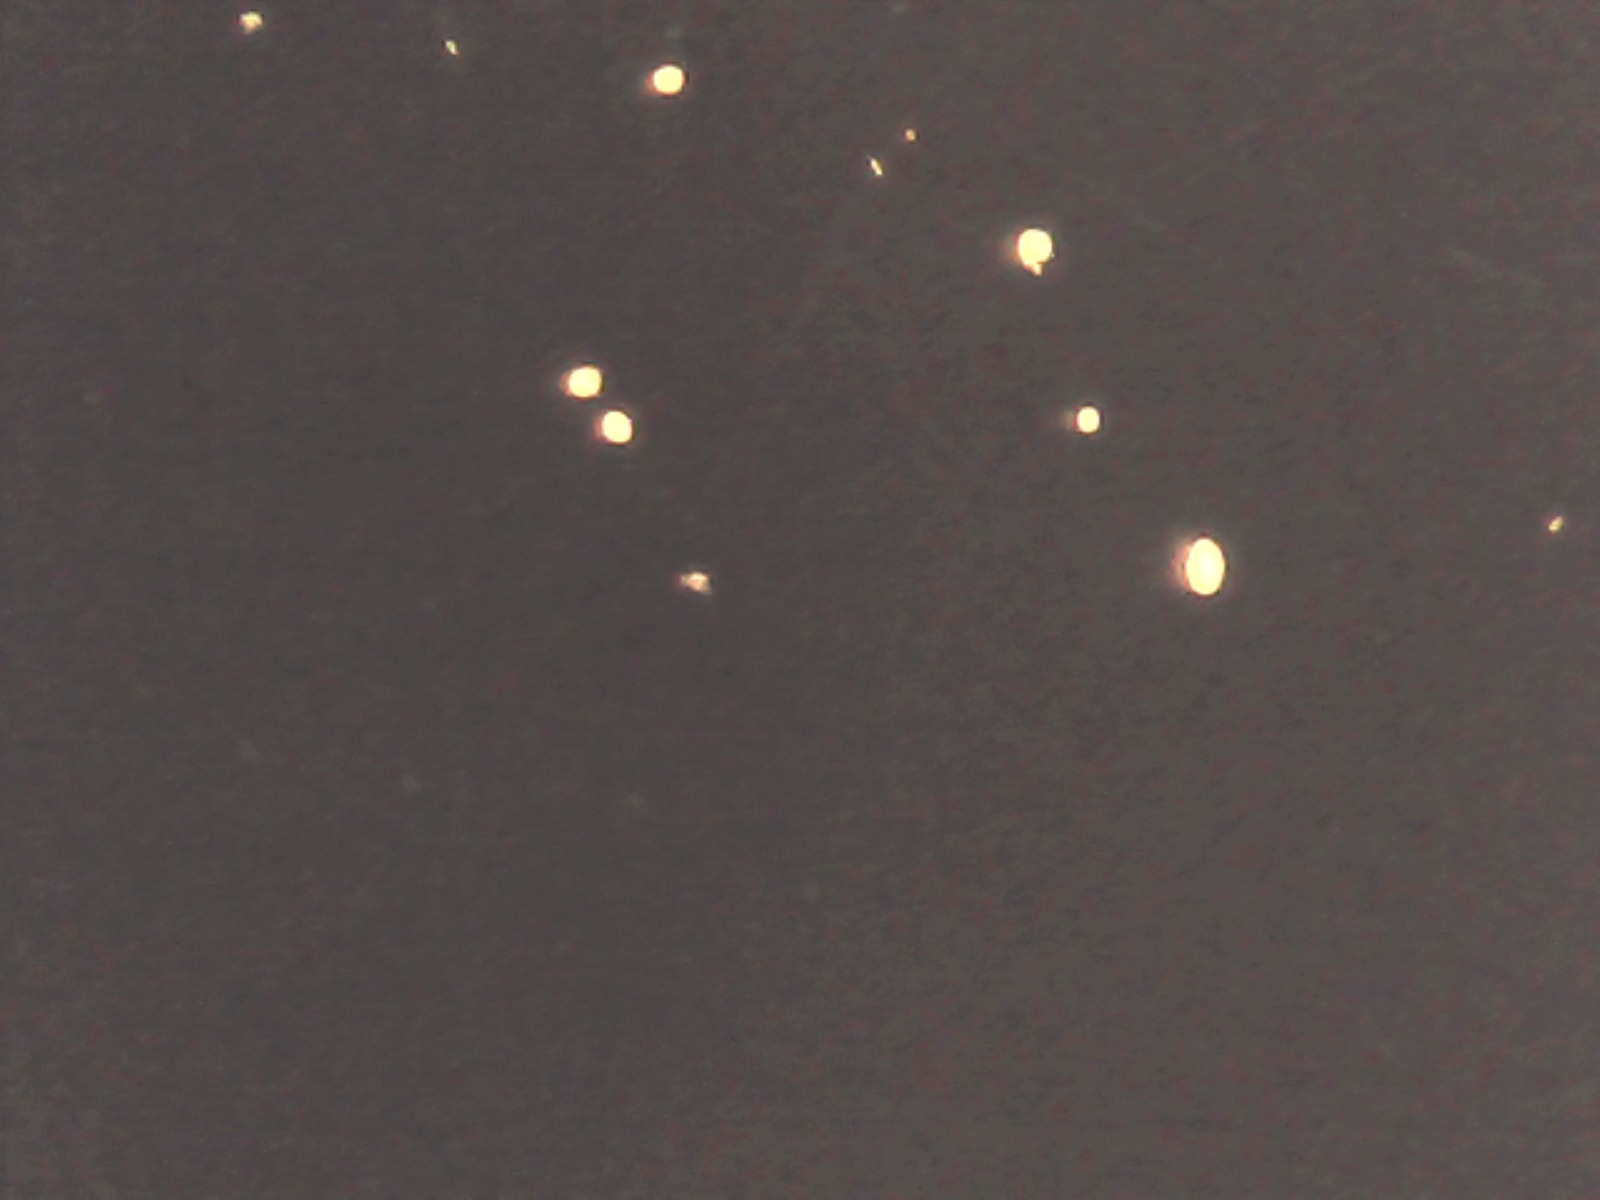
\includegraphics[width=1.00\textwidth]{billeder/software/1.jpg} % Left picture
\end{minipage} \hfill
\begin{minipage}[b]{0.3\textwidth} \centering
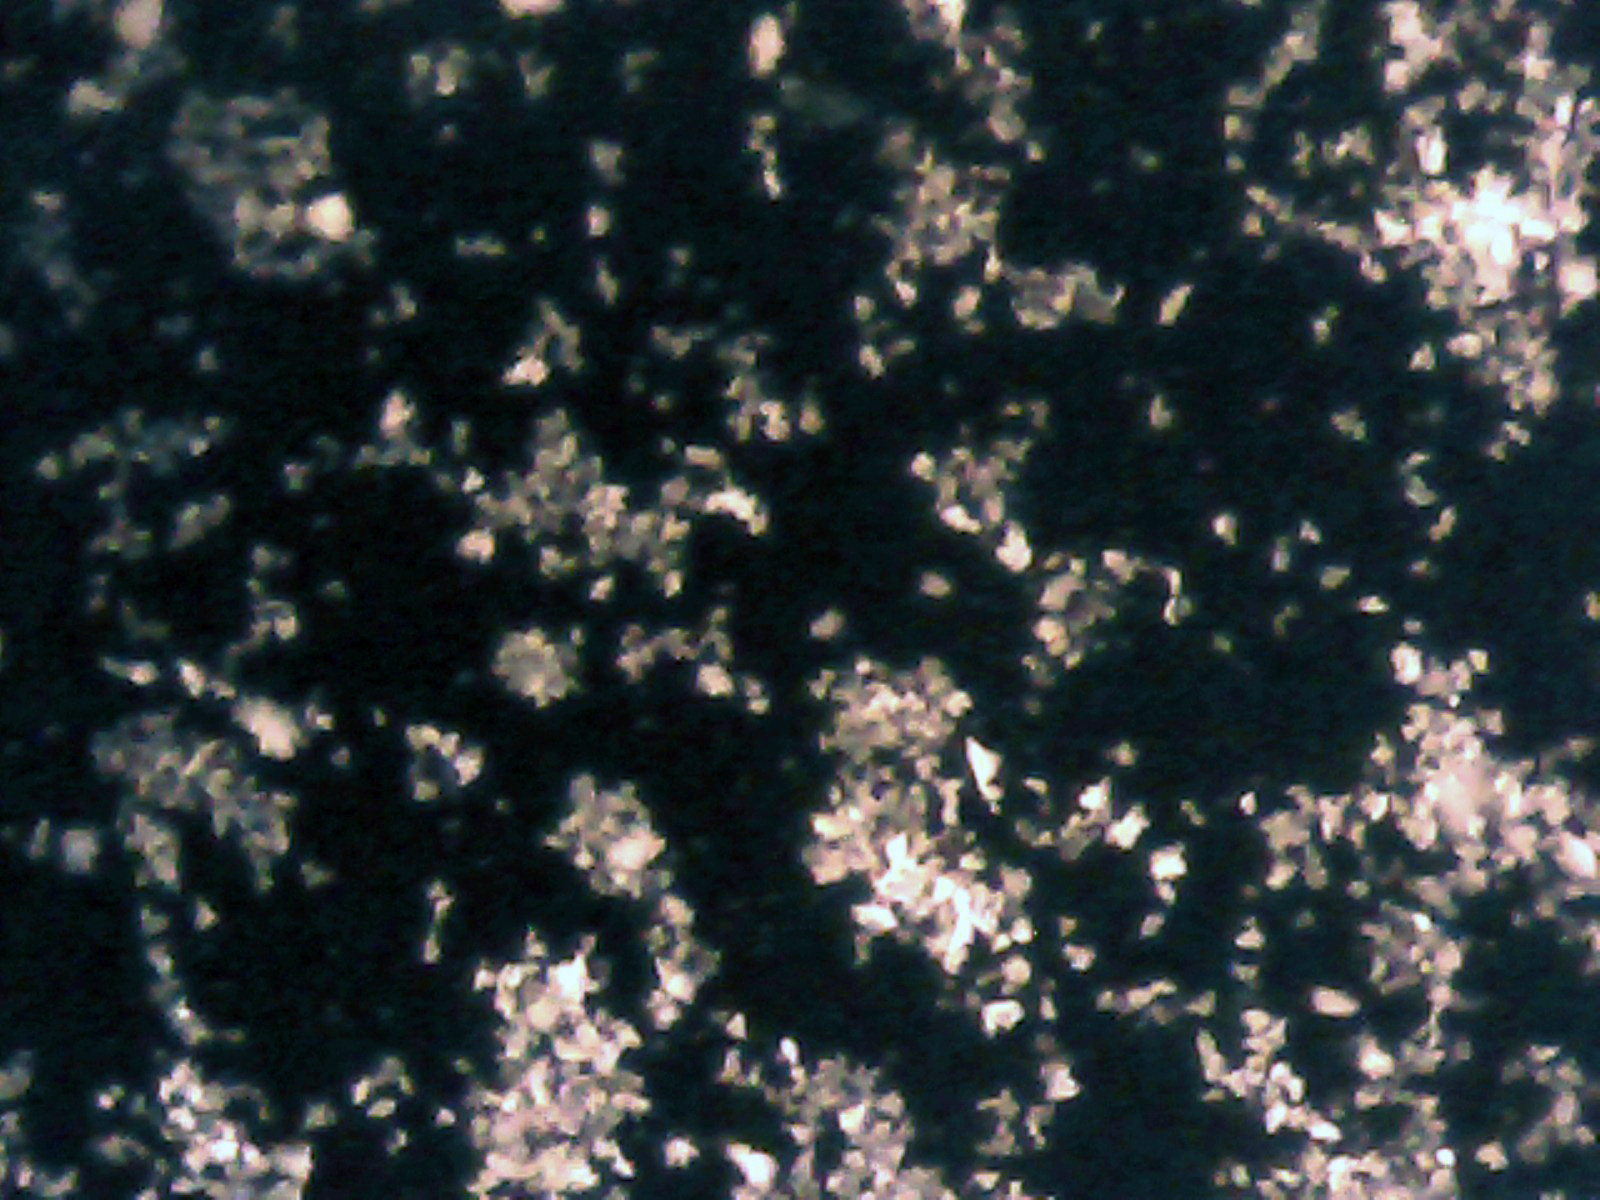
\includegraphics[width=1.00\textwidth]{billeder/software/2.jpg} % Right picture
\end{minipage} 
\hfill
\begin{minipage}[b]{0.3\textwidth} \centering

\includegraphics[width=1.00\textwidth]{billeder/software/3.jpg} % Right picture
\end{minipage} \\  % Captions og labels
\begin{minipage}[t]{0.3\textwidth}
\caption{Billede indeholdende langerhanske øer} % Left caption and label
\label{fig:img1}
\end{minipage} \hfill
\begin{minipage}[t]{0.3\textwidth}
\caption{Billede indeholdende ekstra væv} % Right caption and label
\label{fig:img2}
\end{minipage}
\hfill
\begin{minipage}[t]{0.3\textwidth}
\caption{Baggrundsbillede} % Right caption and label
\label{fig:img3}
\end{minipage}
\end{figure}

\textbf{Fase 1}

Segmenteringen af langerhanske øer sker ud fra billede 1 \ref{fig:img1}, hvor funktionen circleFinder anvendes til at finde centrum og radius på af de fundne celler. Resultatet af circlefinder segmenteringen er vist i fiugr \ref{fig:circlefinder}

 \begin{figure}[H]
	\centering
	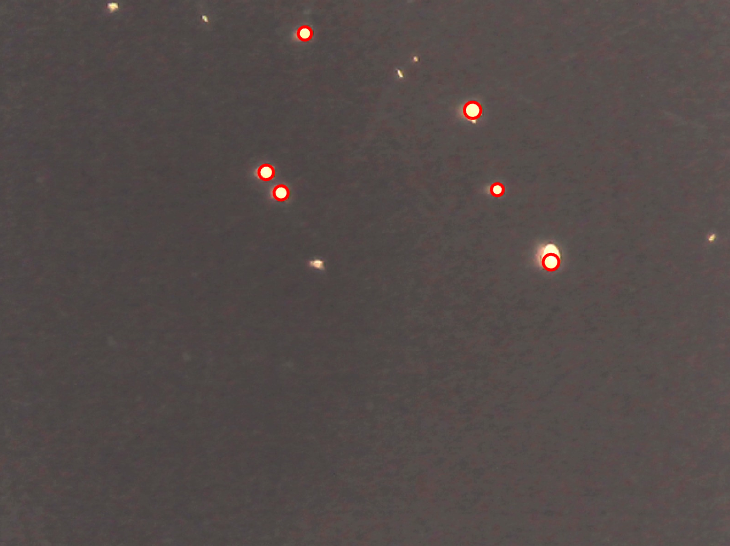
\includegraphics[width=0.5\textwidth]{billeder/software/circlefinder.png}
	\caption{Circlefinder til ø detektion}
	\label{fig:circlefinder}
\end{figure}

Circlefinder funktionen giver følgende funktion, som kan anvendes til at detektere cirkler med. Parametrene Sensitivty og edgeThreshold beskriver, hvor cirkulære objekterne er og generelt hvor følsom algoritmen er. Som det ses på figur \ref{fig:circlefinder} findes der kun én cirkel pr. ønsket ø.
\begin{lstlisting} 
detectCircles = @(x) imfindcircles(x,[12 30], ...
	'Sensitivity',0.8500, ...
	'EdgeThreshold',0.20, ...
	'Method','PhaseCode', ...
	'ObjectPolarity','Bright');
[centers, radii, metric] = detectCircles(im);
\end{lstlisting} 


\textbf{Fase 2}

I anden fase bliver det ekstra væv segmenteret ud fra billede 2 (figur \ref{fig:img2}). Til dette er der anvendt Color Threshold appen i Matlab. Ved hjælp af denne app er der lavet en funktion, som opretter en logisk maske af det ekstra væv. Opsætningen i appen er vist i figur (REF) \fxnote {Indsæt figur}. Yderligere er der anvendt morfologiske operationer til at fjerne uønskede objekter fra masken, samt fjerne støj. Til at fjerne uønskede objekter er funktionen \textit{bwareafilt} anvendt, med parametrene 150 og 500. Dette fjerner alle objekter under 150 og over 500 sammenhørende pixels. Til at udfylde huller i de enkelte objekter er funktionen \textit{imfill} brugt. 

\textbf{Fase 3}

I fase 3 sker selve flow simuleringen. Flowsimuleringen er opbygget på den måde, at den består af henholdvis en sekvens indeholdende en langerhansk ø efterfulgt af en sekvens uden en ø. I selve programmet indlæses et nyt billede hvert 0,1 sekund. Derfor skal der generes en passende mængde billeder, som programmet kan indlæse. Fase 3 er implementeret så der minimum genereres 252 eller maksimalt 432 billeder, hvilket giver en samlet sekvenslængde på 25,2 eller 43,2 sekund. Grunden til at antallet af billeder varierer er at længden af sekvensen uden en langerhansk ø bestemmes udfra en random variabel. Dette gøres for, at simulere at det kan være variabel tid mellem en ny ø kommer i gennem slangen. I scriptet genereres der i alt 18 fulde sekvenser. Det betyder, at der passerer i mellem 25 og 43 øer i minuttet. Antallet af øer der passere pr. minut er bestemt ud fra formel \ref{formular:isletprmin}: 
\begin{align}
\frac{18}{\frac{n}{10}} * 60 = \text{Antal øer pr. minut}
\text{ , hvor n er antallet af billeder i sættet}
\label{formular:isletprmin}
\end{align} 
I figur \ref{fig:boxplot} er vist et boxplot som viser distributionen af hvor mange øer der passerer i minuttet. Det ses at medianen ligger over 30 øer pr. minut, hvilket betyder at der i gennemsnit vil komme over 30 øer pr minut. De 30 øer pr. minut stammer fra hastighedskravet fra systemets kvalitetskrav (\ref{subsec:qa}).

 \begin{figure}[H]
	\centering
	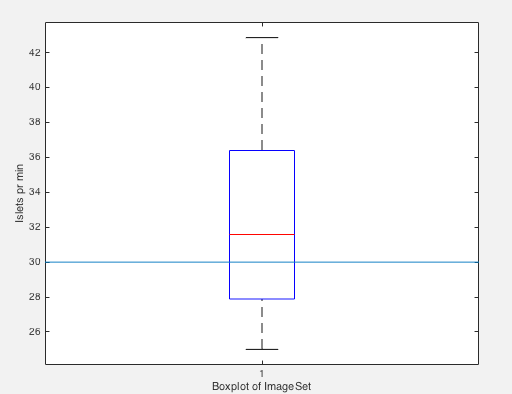
\includegraphics[width=0.5\textwidth]{billeder/software/boxplot.png}
	\caption{Boxplot af distrubutionen af øer pr. minut}
	\label{fig:boxplot}
\end{figure}

Selve flowsimuleringen sker i et for loop. Først udvælges en tilfældig celle ved hjælp af randi (uniform fordelt random variabel). I for loopet opdateres dens center position ud fra 2 variabler (newXPos og newYPos). X positionen springer med et fast interval for hver iteration (160 px). Inden for loopet fastsættes start positionen for cellen med \textit{randi}, som giver et tal mellem 0 og 1200 px (højden på billedet). Herefter opdateres den nye Y position ved hjælp af randn (normal fordelt random variabel) med middelværdi sat til startpositionen og en standard afvigelse på 50 pixels. I figur \ref{fig:flowsim} er flow simulationen illustreret for de i alt 18 sekvenser, med en graf for hver celle. Det ses at cellen flytter sin Y position tilfældigt, mens X positionen springer med et fast interval for hver iteration i for loopet.

\begin{figure}[H]
	\centering
	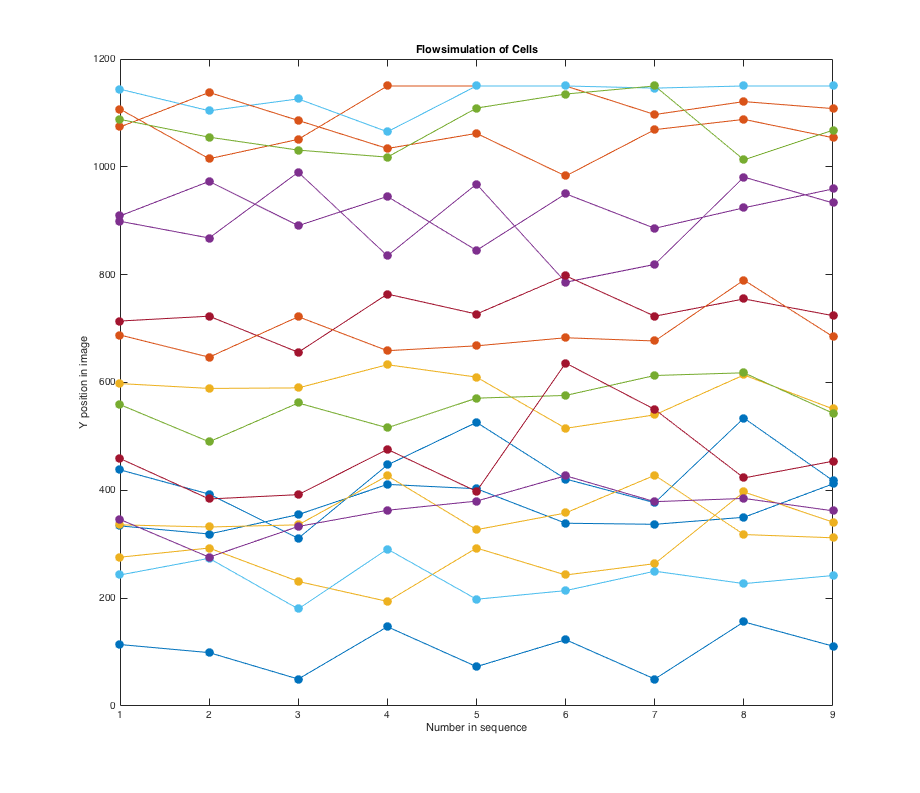
\includegraphics[width=0.5\textwidth]{billeder/software/Simulation.png}
	\caption{Illustration over flow simuleringen}
	\label{fig:flowsim}
\end{figure}

Efter generering af ny x og y position oprettes en maske for cellen ved brug af funktionen createCirclesMask. Til at indsætte cellen i baggrundsbilledet indekseres baggrundsbilledet med masken for cellen, så gråtoneværdierne fra det oprindelige billede indsættes.

Yderligere er der tilføjet tilfældig støj til billedet i form af “Salt and pepper” og gausisk hvid støj. Her er Matlab funktionen \textit{imnoise} anvendt. 

Masken med ekstra væv flyttes for hver iteration med funktionen \textit{circshift}, som bit shifter arrayet cirkulært. Parametrene definerer antallet af rækker og kolonner arrayet skal shiftes.  Antallet af kolonner er fastdefineret til 160 px, mens rækkerne skiftes efter en normalfordelt random variabel med mean på 0 og standard afvigelse på 50 pixels. Nedenstående figur \ref{fig:histfit} viser fordelingen af antallet af rækker der flyttes. På figur \ref{fig:histfit} er der vist markører for standard afvigelsen ($\sigma$) og $2*$standard afvigelsen ($2\sigma$) for hver side af mean. I mellem $-\sigma$ og $\sigma$ er der 68,26 \% sandsynlighed for, at den nye Y position ville ligge inden for dette område. For 2 sd afvigelse ($2\sigma$) er der 95,45 \% for, at den nye Y position vil ligge inden for dette område.

\begin{figure}[H]
	\centering
	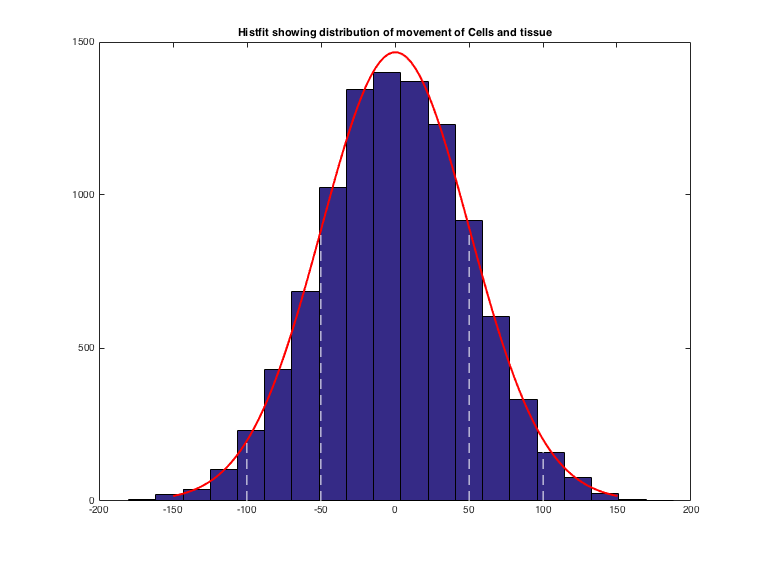
\includegraphics[width=0.5\textwidth]{billeder/software/histfit.png}
	\caption{Histogram over fordelingen af ny Y position}
	\label{fig:histfit}
\end{figure}

Det endelige resultat af billedegeneringen er vist i figur \ref{fig:finalresult}. Til at illustrere hvordan øen flytter sig er der tilføjet en graf, som viser hvordan dens position ændres for hver iteration. Cellen er markeret med en rød ring på billedet.

\begin{figure}[H]
	\centering
	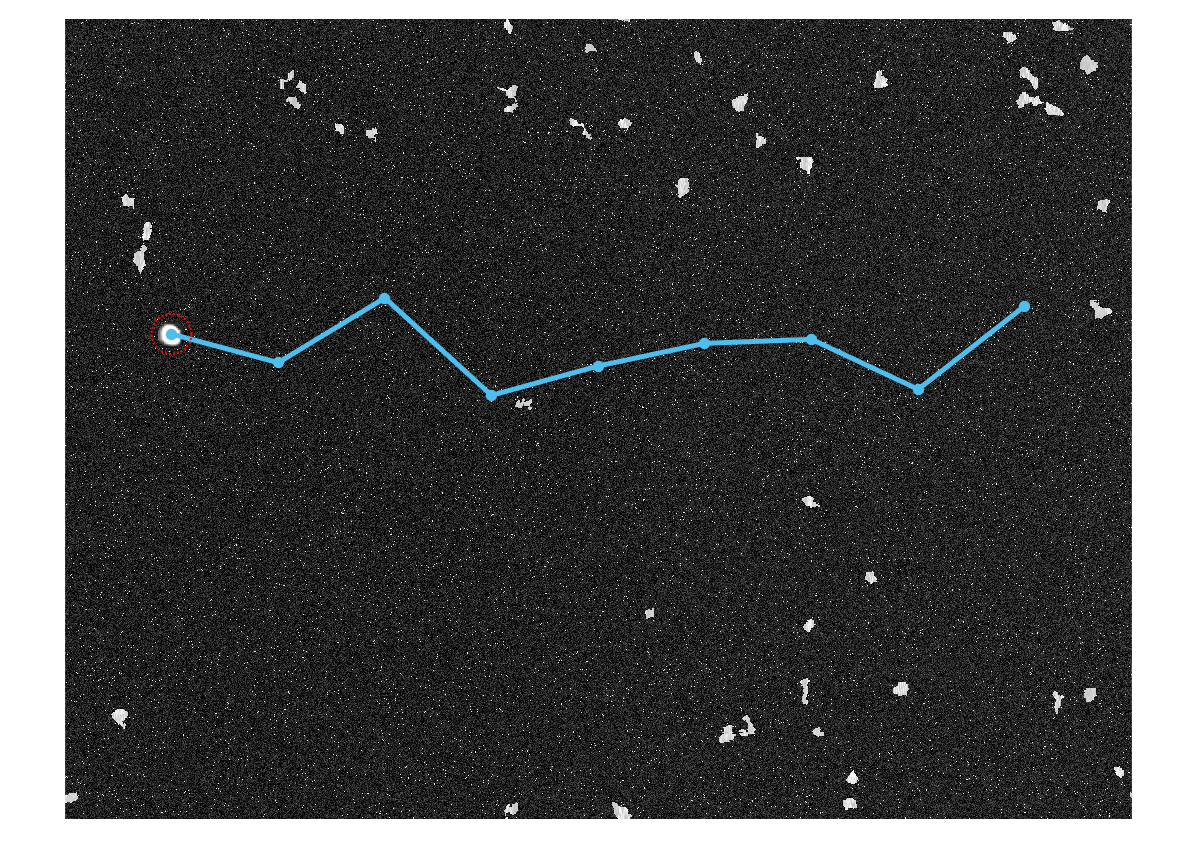
\includegraphics[width=0.7\textwidth]{billeder/software/final.png}
	\caption{Endelige resultat for flowsimulering}
	\label{fig:finalresult}
\end{figure}

Implementeringen af scriptet er vedlagt i bilag \fxnote{Indsæt referencer til bilag}  

\subsubsection{Det samlede kredsløb}
Til at samle de forskellige hardware deles kredsløb, er der lavet et samlet printkort til dette. Se diagrammet for printet på figur XX

\subsubsection{Det færdig print layout}
Printkortets layout er udarbejdet i \textit{Eagle}, hvor lagene er eksporteret til \textit{gerber} filer. Filerne er sendt til printfremstilling ved ingeniør højskolens værksted. Nedenfor på figur XX kan layoutet ses i \textit{Eagle}

\subsection{Ikke-elektroniske dele}
De ikke-elektroniske dele, består af beholdere, slanger og adaptere. I projektet er der fokuseret på opløsningsbeholderen, hvor der er indkøbt en 250ml beholder med et specielt låg. Igennem låget går der en teflonslange, for at tætne denne tilslutning er der en forskruning der både aflaster og tætner i låget. I låget er der også et luftfilter, som forhindre støv og andre små partikler for at komme ned i opløsningen. Filteret skal være der for at undgå dannelse af undertryk i beholder, når pumpen suger opløsningsvæsken igennem systemet. Da teflonslangen ikke er eftergivende, er der brugt silikoneslanger til stykket igennem pumpen og resten af systemet. Det er der fordi teflonslangen er for hård til, at pumpen kan sammenpresse den og derved skabe flow i opløsningen. For at kunne gå fra teflonslangen til silikoneslangen er der brugt en adapter. Se styklisten mm. i projektdokumentation afsnit XX.
\fxnote{illustration af de ikke-elektroniske dele gælder også i dokumentationen}

\section{Simuleringsvæske}
\label{sec:simuleringsv}
Da de langerhanske øer ikke er lettilgængelig, har det været nødsaget at finde et objekt til at agere aktør for cellerne. Simuleringsvæsken skal bruges til at teste de mekaniske dele, samt tidsintervallet mellem kameraet og ventilen. Egenskaberne af de langerhanske øer der er brugt til at finde simuleringsvæsken er at de er runde og lyse, størrelsen, samt at de bundfælder i colleganse opløsningen. Der har været to iterationer for at finde en aktør for cellerne, den første har bestået i at finde perfekte runde og hvide objekter med en $massefylde<1$. Til dette blev der brugt polysterene, som er lettilgængelig, samt runde, hvide og kan fåes med en massefylde lige over en \fxnote{reference til bedre side end wiki?}. Dog blev det fundet svært at finde polysterene kugler i størrelsen 0.1-0.3mm, derfor blev der skabt kontakt til forhandlere af flamingo kugler. Dog var de tilsendte kugler for store, samt flød oven på. 

Den anden iteration bestod i at finde et biologisk materiale, hvor ved faktorerne runde og hvide blev nedprioriteret for at finde et objekt. For at finde en celle aktør med lettilgængelighed blev plantefrø den næste mulighed. Trods begrænset data omkring plantefrø, lykkes det gruppen at finde plantefrø i størrelsen 0.1-0.3mm vha. forhandlere af plantefrø og andre eksperter \fxnote{referencer til mail}. De indkøbte frø består af timian frø og rævehale frø \fxnote{indsæt billeder}. Udover de indkøbte frø kan der ved videre bearbejdelse af projektet overvejes transparent testa (tt4 mutant) frø. De skulle i følge \textit{Carsten Meier} være hvide, forholdsvis runde, dog er de ikke lige så tilgængelige, som de allerede indkøbte frø. Dette har været grunden til, at de ikke er brugt i projektet ind til nu. Derfor består den anvendte simuleringsvæske af, demineraliseret vand og timian plantefrø som aktør for de langerhanske øer.  
 
\section{Aceepttest af produktet} 
 beskriv ikke bestået krav og hvorfor de ikke er det. beskriv også bestået krav. reference til udført accepttest.
\newpage
\section{Cost-benefit analyse}
Dette afsnit indeholder cost-benefit analysen, som belyser hvilke omkostninger der er forbundet med sortering af langerhanske øer. Analysen sammenligner omkostningerne forbundet med den manuelle sorteringsproces og den automatiserede metode. Formålet med analysen er, at beregne hvad stk. prisen pr. ø er ved henholdsvis den ene og den anden metode. Dette anvendes til at give en tidshorisont for hvornår en investering af den automatiserede løsning vil være tjent hjem igen. Udgangspunktet for analysen bygger på det tidsmæssige forbrug der er forbundet med isolering af et batch på 400 øer fra mus. 

Fælles for begge sorteringsmetoder er, at der fortsat foretages manuel perfusion og nedbrydning og vaskning af pankreas. Nedenstående tabel opsummere hvilke basisudgifter der er forbundet ved disse processer. Timelønnen er beregnet ud fra en PhD studerendes månedsløn på 25.040 kr \citep{phdwage}.
\begin{center}
		\begin{longtable}{ | m{6cm} | m{1.5cm} | m{1.5cm} | m{3cm}| } 
			\hline
			 &\textbf{Antal} & \textbf{Pris} & \textbf{Total}\\ 
			\hline
			 \textbf{Mus} & 6 stk & 60 kr & 360 kr\\ 
			\hline
			 \textbf{Tid for perfusion} & 1 time & 171,62 kr & 171,62 kr\\ 
			\hline
			\textbf{Tid for nedbrydning + vask} & 1 time & 171,62 kr & 171,62 kr\\ 
			\hline	
			\textbf{Total} &  &  & \textbf{703,24 kr}\\ 
			\hline
			\caption{Basis omkostninger for sorteringsproces}
			 		\end{longtable}
\end{center}
Nedenstående tabel \ref{tab:sortcost} viser, hvilke omkostninger der er forbundet med selve isoleringsprocessen af de langerhanske øer. Den halve time der bruges ved den automatiske metode er et estimat af hvad der skal bruges på påfyldning af beholdere og start af sorteringsproces. 
\begin{center}
		\begin{longtable}{ | m{6cm} | m{1.5cm} | m{1.5cm} | m{3cm}| } 
			\hline
			 &\textbf{Antal} & \textbf{Pris} & \textbf{Total}\\ 
			\hline
			 \textbf{Tid manuel} & 6 timer & 171,62 kr & 1029,73 kr\\ 
			\hline
			 \textbf{Tid automatisk} & 0,5 timer & 171,62 kr & 85,81 kr\\ 
			\hline
			\caption{Omkostninger ved sortering af langerhanske øer}
			\label{tab:sortcost}
			 		\end{longtable}
\end{center}
Omkostningerne ved de to sorteringsmetoder er opsummeret i tabel \ref{tab:totalcost}, herunder en samlet pris for et batch på 400 øer, og en stk. pris pr. ø for hver sorteringsmetode.
\begin{center}
		\begin{longtable}{ | m{8cm} | m{2.25cm} | m{2.25cm} | } 
			\hline
			 &\textbf{Manuelt} & \textbf{Automatisk} \\ 
			\hline
			 \textbf{Basis omkostninger} & 703,24 kr & 703,24 kr \\ 
			\hline
			 \textbf{Isoleringsomkostninger} & 1029,73 kr & 85,81 kr \\ 
			\hline
			\textbf{Total pris for sortering} & 1732,97 kr & 789,05 kr \\ 
			\hline
			\textbf{Pris pr. ø ved batch på 400 stk} & 4,33 kr & 1,97 kr \\ 
			\hline
			\caption{Opsummering af omkostninger for sorteringsprocesen for de to sorteringsmetoder}
			\label{tab:totalcost}
			 		\end{longtable}
\end{center}

Da der er forbundet omkostninger ved en investering i et system til automatisk isolering, er udgifterne til den udviklede prototype opsummeret i tabel \ref{tab:prototypecost}. I tabellen er de enkelte hardware komponenters pris noteret, samt hvad en licens til Matlab koster. Herudover er der vurderet en profit på 400 \% af udgifterne til hardware komponenter og Matlab licens. Denne udgift dækker udgifter til support og vedligehold, produktion, monteringsomkostninger, garanti og udvikling. Som det ses i tabellen er udgiften til den udviklede prototype beregnet til 86175 kr.
\begin{center}
		\begin{longtable}{ | m{9.5cm} | m{3.5cm} | } 
			\hline
			  & \textbf{Pris} \\ 
			\hline
			Kamera & 400 kr \\ 
			\hline
			 Ventil & 845 kr\\ 
			\hline
			Pumpe & 80 kr  \\ 
			\hline
			Arduino & 150 kr \\ 
			\hline
			Andet hardware & 210 kr \\ 
			\hline
			Beholdere + slanger & 425 kr \\ 
			\hline
			3d print & 125 kr \\ 
			\hline
			Matlab licens & 15000 kr \\
			\hline
			Profit på 400\% & 68940 kr \\	
			\hline
			\textbf{Total pris} & \textbf{86175 kr} \\		
			
			\hline
			\caption{Udgifter til automatiseret system}
			\label{tab:prototypecost}
			 		\end{longtable}
\end{center}


\newpage
Til at illustrere og sammenligne udgifterne for de to sorteringsmetoder viser figur \ref{fig:costbenefit} udgiften over tid. Figuren viser omkostningerne set over en periode på 2 år, ved at der sorteres et batch pr. uge.

\begin{figure}[H]
	\centering
	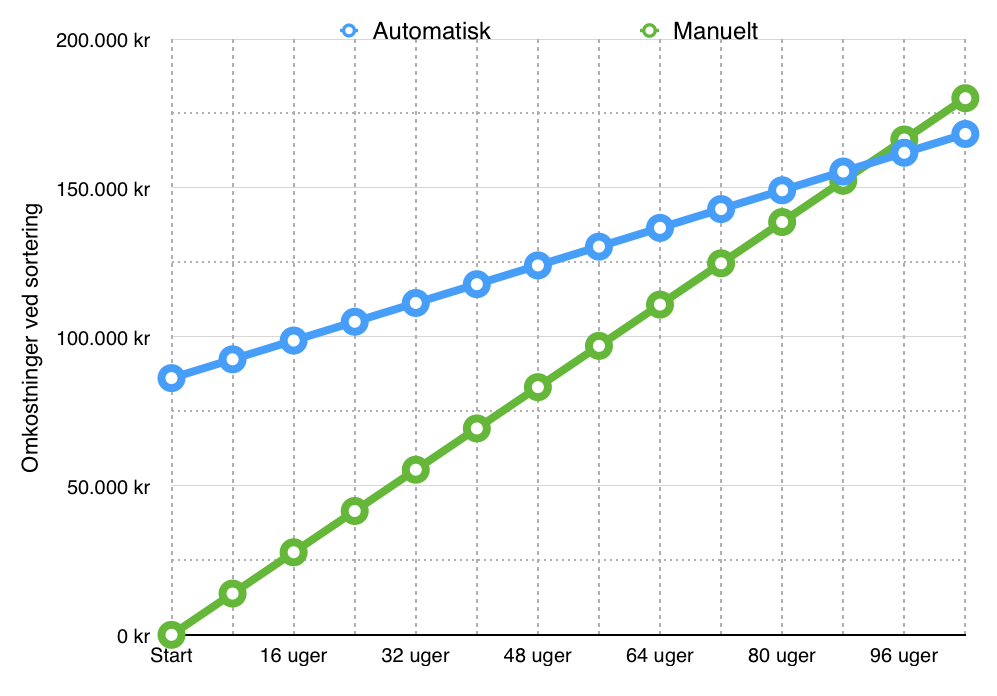
\includegraphics[width=1\textwidth]{billeder/Hovedrapport/costbenefit2.png}
	\caption{Udvikling i omkostninger }
	\label{fig:costbenefit}
\end{figure}

Af figur \ref{fig:costbenefit} ses det, at efter 92 uger overstiger omkostningerne ved den manuelle sorteringsproces de omkostninger der er ved den automatiske, og investeringen vil her være tjent hjem. 





Andre ting?